\begin{minipage}[t]{100mm}
\vspace{3mm}

\section*{Løsning af søndagens opgave}
Den røde kontakt spiller ingen rolle i løsningen andet end at blive skiftet hvis en fange ønsker at undgå a skifte den grønne kontakt. Den røde kontakt udelades derfor i følgende beskrivelse af løsningen.
 \\ \\
Fange 1 har to variable: FørsteBesøg der starter som ``sand'', og AndresBesøg der starter som $0$. Når fange 1 besøge celle 0 foretages følgende: Hvis FørsteBesøg $=$ ``sand'', sættes FørsteBesøg $=$ ``falsk'', og hvis den grønne kontakt er slukket, tændes den. Hvis FørsteBesøg $=$ ``falsk'', betragtes den grønne kontakt: Hvis den grønne kontakt er slukket, tændes den og der lægges én til AndresBesøg, ellers gør fange 1 intet. Hvis AndresBesøg $=43$ i slutningen af besøget, ved fange 1 at alle har været igennem celle 0.
 \\ \\
Alle andre fanger har én variabel: AntalGrønne der starter som $0$. Når en sådan fange besøger celle 0 gøres følgende: Hvis den grønne kontakt er tændt, og AntalGrønne $<2$, så slukker fangen den grønne kontakt og lægger 1 til AntalGrønne, ellers gør fangen intet.

\section*{Dagens sætning - Pizza Sætningen}
Hvis en rund pizza bliver delt i $8, 12, 16, \dots$ slices ved fra et vilkårligt punkt på pizzaen at inddele den i slices med samme vinkel, så vil man, hvis man spiser hvert andet stykke rundt, have spist halvdelen af pizzaen.
\\
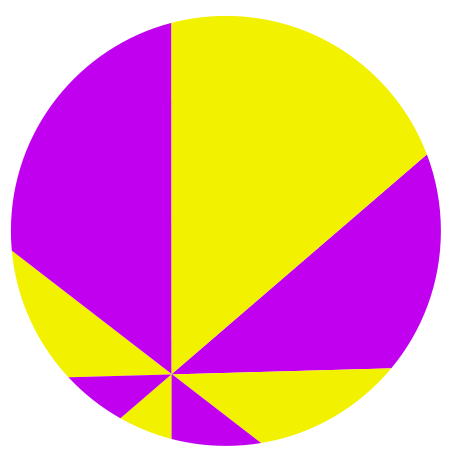
\includegraphics[width=\textwidth]{Pizzathm.png}
\end{minipage}
